%%%% Proceedings format for most of ACM conferences (with the exceptions listed below) and all ICPS volumes.
\documentclass[sigconf]{acmart}
%%%% As of March 2017, [siggraph] is no longer used. Please use sigconf (above) for SIGGRAPH conferences.
\settopmatter{printacmref=false} % Removes citation information below abstract
\renewcommand\footnotetextcopyrightpermission[1]{} % removes footnote with conference information in first column
\pagestyle{plain} % removes running headers


\usepackage{booktabs} % For formal tables


\newcommand{\luke}[1]{{\color{blue} #1}}
\newcommand{\para}[1]{\vspace{0.08in}\noindent\textbf{#1 }}

% Squished list environment to save space
\newcommand{\squishlist}{
 \begin{list}{$\bullet$}
  { \setlength{\itemsep}{0pt}
    \setlength{\parsep}{2pt}
    \setlength{\topsep}{2pt}
    \setlength{\partopsep}{0pt}
    % \setlength{\labelwidth}{1em}
  }
}
\newcommand{\squishend}{\end{list}}


\begin{document}
\title{ReBBR: Reproducing BBR Evaluation Results}
% \subtitle{Extended Abstract}

\author{Luke Hsiao}
\affiliation{%
  \institution{Stanford University}}
\email{lwhsiao@stanford.edu}

\author{Jervis Muindi}
\affiliation{%
  \institution{Stanford University}}
\email{jmuindi@stanford.edu}


\begin{abstract}
This report describes an attempt to reproduce one of the key
findings from the BBR Paper by Cardwell et al. The primary
result we pursue is performance of BBR compared to CUBIC in
networks that have non-negligible packet loss. As reported
in the original paper, we find that in our preliminary exploration,
CUBIC has poor performance for loss rates above 0.1\% whereas BBR is able
to provide higher utilization of the network up to much high loss rates.
\end{abstract}


% \keywords{ACM proceedings, \LaTeX, text tagging}

%% Used in some conference proceedings e.g. sigplan and sigchi
% \begin{teaserfigure}
%   \includegraphics[width=\textwidth]{sampleteaser}
%   \caption{This is a teaser}
%   \label{fig:teaser}
% \end{teaserfigure}

\maketitle

% !TEX root = ../main.tex

\section{Introduction}
In this report, we attempt to validate the experimental results of ``BBR:
Congestion-based Congestion Control''~\cite{cardwell2016bbr}. We start
by looking at the goals, motivations and results from the BBR paper.

\para{Goals}
\emph{What was the original paper trying to solve?}

The original paper was trying to find a congestion control approach
that would stay as close as possible to optimal network operating point
in various network conditions. The network link is operating at the optimal
point when bandwidth utilization is maximized and latency and loss are
minimized, as shown by Leonard Kleinrock in 1979~\cite{kleinrock1979power}.
Furthermore, Jeffrey Jaffe proved that a distributed algorithm that converged
to this optimal point was an impossibility~\cite{jaffe1981flow}.

Loss-based congestion control operates by delivering full
bottleneck bandwidth at the cost of high delay and frequent packet loss.
Furthermore, Cardwell et. al. observed that because Round Trip Propagation delay
(RTprop) and Bottleneck bandwidth (BtlBw) could be inferred from traces,
measurements over time could result in an algorithm which converged with
high probability to the optimal operating point. BBR is an algorithm that
seeks to converge to this optimal point.


\para{Motivation}
\emph{Why is the problem important/interesting?}

At a high level, the Internet could be moving data much more efficiently.
For example, cellular users can experience delays of seconds to minutes and
even multi-Gbps infrastructure may deliver data at a few Mbps when transmitting
over intercontinental distances. In addition, traditional congestion control
algorithms such as CUBIC have a tough time operating efficiently when there
is non-negligible packet loss in the network. This limitation comes from
CUBIC's use of packet loss as a signal for congestion, which can unnecessarily
hinder throughput leading to poor performance.

Importantly, these limitations are not fundamental, but rather are a result
of particular implementation choices made in designing TCP congestion control.
In the original paper, the BBR authors seek to find an alternative to loss-based
congestion control, in an effort to mitigate many of these issues.

The problem is particularly interesting because, if successful, we will be able
to utilize the network infrastructure we have much more effectively, while
reducing latency experienced by users, without needing to upgrade or change
the network itself.

\para{Results}
\emph{What did the original authors find?}

The BBR paper describes a new form of congestion control that is based on actual
congestion in the network. The insight from the authors is that their
approach estimates bottleneck bandwidth and the minimum propagation delay
so as to be able to get as close as possible to the ideal operating point of
maximum bandwidth and minimal latency. We highlight a few of the key
results below.

The first finding is that BBR can quickly adopt to changes in bottleneck link
bandwidth. During operation, BBR spends most of its time continuously probing
if more bandwidth has become available. Figure~\ref{fig:bbr3} shows BBR
reacting to a 2x increase and a 2x decrease to bottleneck bandwidth within
about 2 seconds.

\begin{figure}[h]
  \centering
  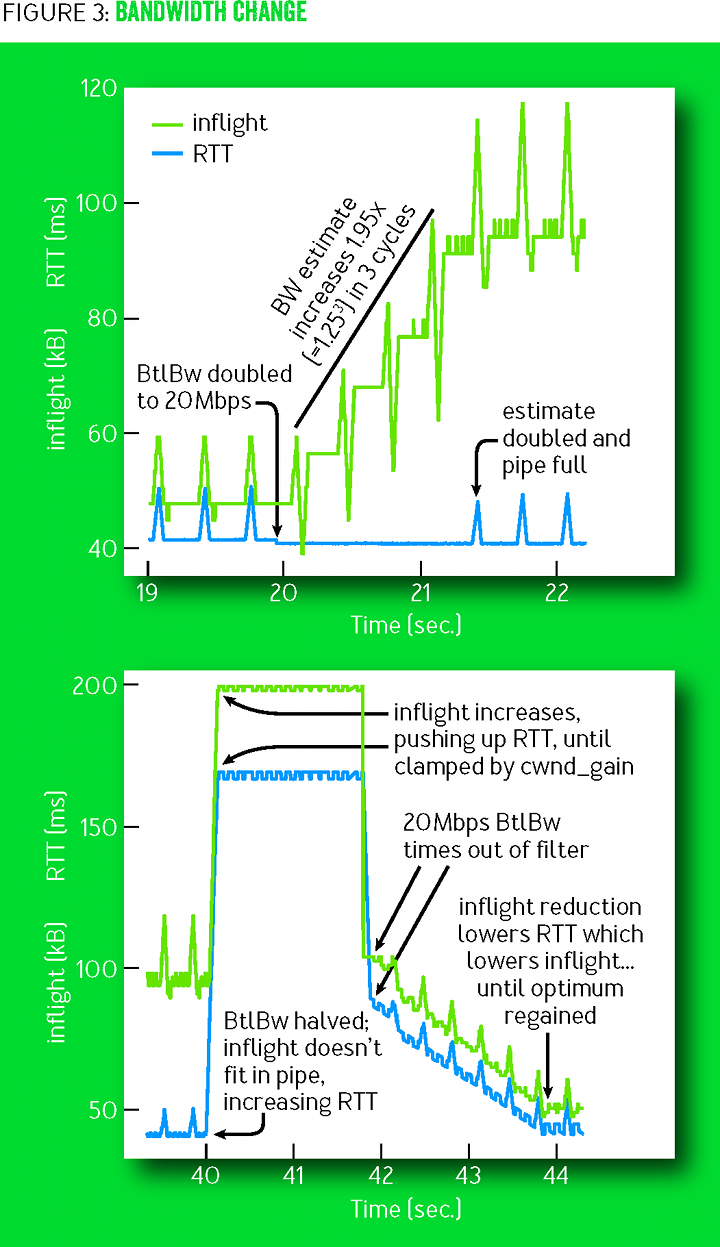
\includegraphics[height=9cm]{./img/bbr_fig3.png}
  \caption{BBR converges to new bottleneck bandwidth at exponential rate.
  This figure is from the original paper.}
  \label{fig:bbr3}
\end{figure}

The second finding is that BBR is able to avoid bloating router buffers
unnecessarily and thus is able to keep RTT at a minimum. This is in contrast to
CUBIC which continues to bloat a the bottleneck buffer until it observes a
packet loss event from overflowing the buffer. Figure~\ref{fig:bbr5} illustrates
hoe CUBIC and BBR behave in this regard.

\begin{figure}[h]
  \centering
  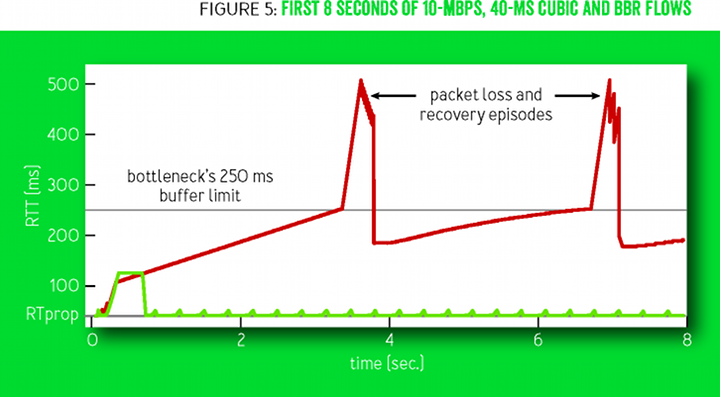
\includegraphics[width=1.0\columnwidth]{./img/bbr_fig5.png}
  \caption{BBR avoids bloating router buffer unlike CUBIC. Figure from original paper.}
  \label{fig:bbr5}
\end{figure}

Third, and one of the most interesting results, is that BBR outperforms
CUBIC for non-negligible loss rates. Figure~\ref{fig:bbr8} shows a graph
showing the performance comparison between BBR and CUBIC for varying loss rates.

\begin{figure}[h]
  \centering
  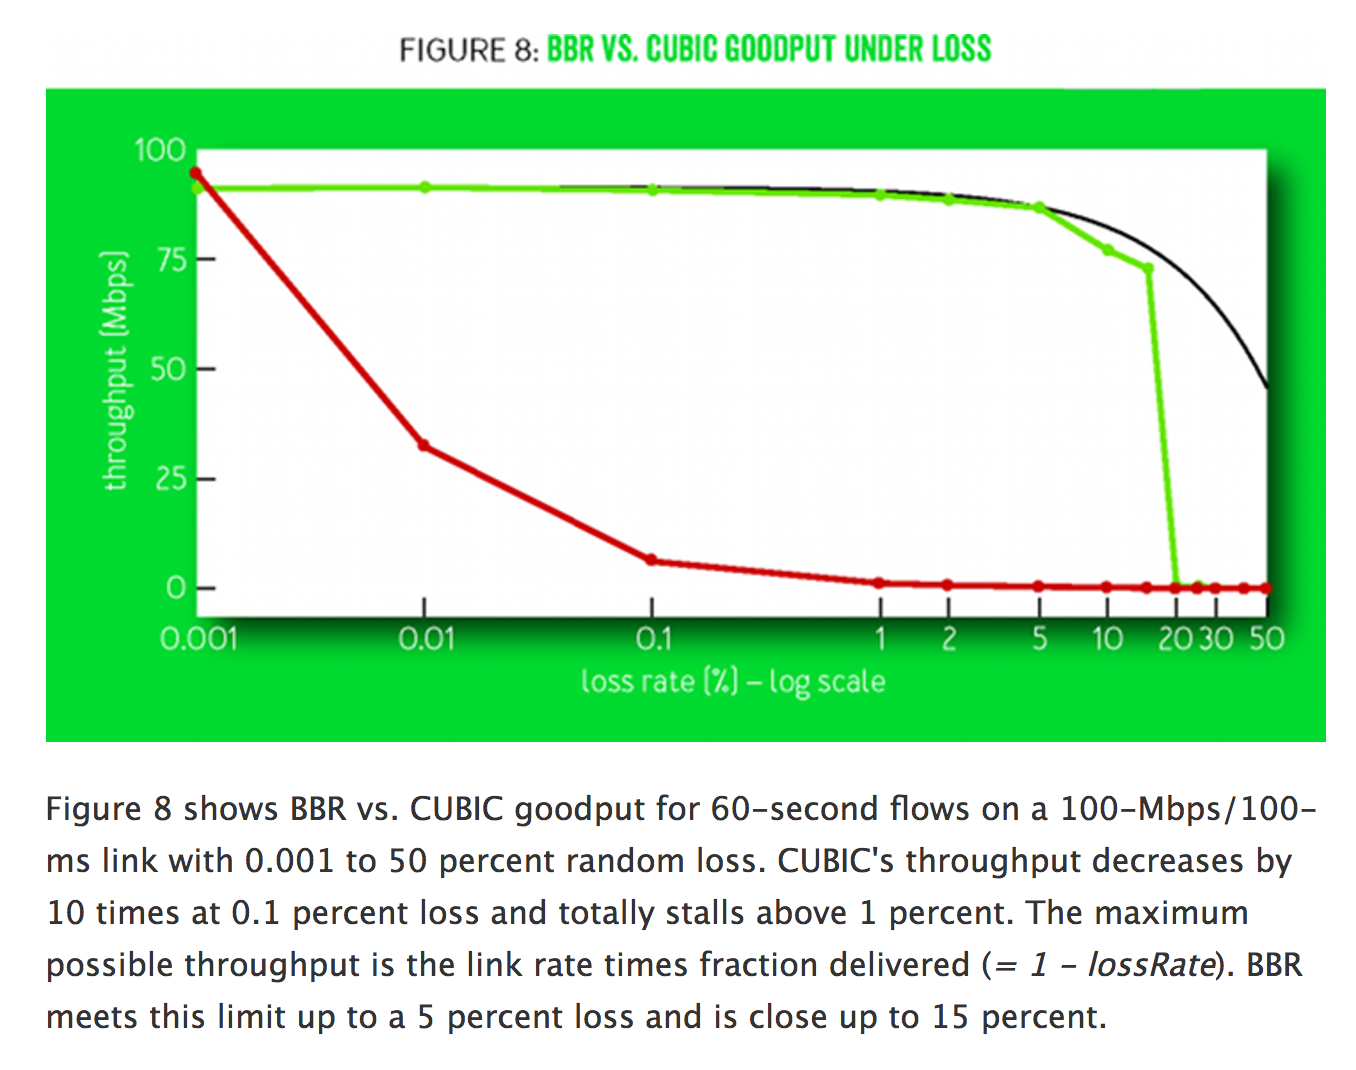
\includegraphics[width=1.0\columnwidth]{./img/bbr_fig8.png}
  \caption{Throughput vs loss rate comparing CUBIC vs BBR. Figure from original paper.}
  \label{fig:bbr8}
\end{figure}

The authors report that Google has had a very good experience deploying BBR
on B4---Google's data center to data center high-speed Wide Area Network built
primarily from commodity switches that have shallow/small memory buffers.
The limited amount of buffering means that there is the occasional packet
loss when there are bursts of incoming packets that arrive at the same time.
After switching to BBR from CUBIC, Google saw throughput improvements ranging
from $2\times$ to $25\times$.

Finally, the authors do acknowledge that there is still work to be done in terms
of how BBR interoperates with existing loss-based congestion controls algorithms
such as CUBIC. In cases where routers have large buffers, CUBIC senders can
drown out BBR. Gracefully mitigating this is an ongoing area of research.

% !TEX root = ../main.tex

\section{Reproducing BBR Evaluation}

\para{Goal} What subset of results did you choose to reproduce?

The main result we focused on reproducing is the comparison between
CUBIC and BBR and how their performance varies across different loss
rate.

This result can be seen in  Figure~\ref{fig:bbr8}.

\para{Motivation} Why that particular choice?

We chose this result because it is a good representative summary
that captures the primary essence of the paper. This is that
loss-based congestion control schemes such as CUBIC are non-optimal
because their use of packet loss as a signal for congestion makes them
very sensitive to any (regular) packet loss that occurs on a path and it
also contributes to buffer bloat which increases latency.




% !TEX root = ../main.tex

\section{Project Status}

The status of the project is that we have completed the setup of a machine with BBR available. This involved
configuring a Linux (Ubuntu) machine with a kernel that included the BBR congestion control algorithm.

In addition, we have been able to write an experiment script in Python that collects data on BBR and CUBIC
throughput performance at varying loss rates. The network emualtor used is MahiMahi. To setup the experiment,
we use a delay shell to simulate a 100ms delay, a loss shell to control the amount of packet loss, and a link
shell to approximate a 100Mbps link.

Once the data collection is complete, the script generates a plot of the performance between BBR and CUBIC.


\para{Plan}
For the remaining days, we need to make the experiment setup run on Google Cloud. Running a machine on Google Cloud
cost a few dollars, so for convienence and for faster iterating, we have been doing our work in a local Linux Ubuntu
VM. The next step is to replicate that setup to run successfully in the Google Cloud.

We would also like to explore how BBR compares to other modern TCP congestion control algorithms
such as VEGAS.

We are also interested on evaluating how does the performance between CUBIC and BBR vary, if at all, when the network
link is running an order of magnitude slower. For example at 10Mbps, 1Mbps, 0.1Mbps (100kbps) and 0.01Mbps (10kbps).
Similarly, it would also be interesting to see the variation when the RTT changes by an order of magnitude. For example
at 0.01s, 0.1s, 1.0s, 10, 60s. Performance on the low bandwidth, high latency links should give insights into
potential benefits of BBR when deployed over slow 2G cellular links.

Finally, we need to write up our final report discussing the results we found.

Admittedly, this is  quite a bit of material and we'll try to get through as much of it as possible, time permitting.



\bibliographystyle{ACM-Reference-Format}
\bibliography{references}

\end{document}
